% Options for packages loaded elsewhere
\PassOptionsToPackage{unicode}{hyperref}
\PassOptionsToPackage{hyphens}{url}
\PassOptionsToPackage{dvipsnames,svgnames,x11names}{xcolor}
%
\documentclass[
  12pt]{article}

\usepackage{amsmath,amssymb}
\usepackage{iftex}
\ifPDFTeX
  \usepackage[T1]{fontenc}
  \usepackage[utf8]{inputenc}
  \usepackage{textcomp} % provide euro and other symbols
\else % if luatex or xetex
  \usepackage{unicode-math}
  \defaultfontfeatures{Scale=MatchLowercase}
  \defaultfontfeatures[\rmfamily]{Ligatures=TeX,Scale=1}
\fi
\usepackage{lmodern}
\ifPDFTeX\else  
    % xetex/luatex font selection
\fi
% Use upquote if available, for straight quotes in verbatim environments
\IfFileExists{upquote.sty}{\usepackage{upquote}}{}
\IfFileExists{microtype.sty}{% use microtype if available
  \usepackage[]{microtype}
  \UseMicrotypeSet[protrusion]{basicmath} % disable protrusion for tt fonts
}{}
\makeatletter
\@ifundefined{KOMAClassName}{% if non-KOMA class
  \IfFileExists{parskip.sty}{%
    \usepackage{parskip}
  }{% else
    \setlength{\parindent}{0pt}
    \setlength{\parskip}{6pt plus 2pt minus 1pt}}
}{% if KOMA class
  \KOMAoptions{parskip=half}}
\makeatother
\usepackage{xcolor}
\setlength{\emergencystretch}{3em} % prevent overfull lines
\setcounter{secnumdepth}{5}
% Make \paragraph and \subparagraph free-standing
\makeatletter
\ifx\paragraph\undefined\else
  \let\oldparagraph\paragraph
  \renewcommand{\paragraph}{
    \@ifstar
      \xxxParagraphStar
      \xxxParagraphNoStar
  }
  \newcommand{\xxxParagraphStar}[1]{\oldparagraph*{#1}\mbox{}}
  \newcommand{\xxxParagraphNoStar}[1]{\oldparagraph{#1}\mbox{}}
\fi
\ifx\subparagraph\undefined\else
  \let\oldsubparagraph\subparagraph
  \renewcommand{\subparagraph}{
    \@ifstar
      \xxxSubParagraphStar
      \xxxSubParagraphNoStar
  }
  \newcommand{\xxxSubParagraphStar}[1]{\oldsubparagraph*{#1}\mbox{}}
  \newcommand{\xxxSubParagraphNoStar}[1]{\oldsubparagraph{#1}\mbox{}}
\fi
\makeatother


\providecommand{\tightlist}{%
  \setlength{\itemsep}{0pt}\setlength{\parskip}{0pt}}\usepackage{longtable,booktabs,array}
\usepackage{calc} % for calculating minipage widths
% Correct order of tables after \paragraph or \subparagraph
\usepackage{etoolbox}
\makeatletter
\patchcmd\longtable{\par}{\if@noskipsec\mbox{}\fi\par}{}{}
\makeatother
% Allow footnotes in longtable head/foot
\IfFileExists{footnotehyper.sty}{\usepackage{footnotehyper}}{\usepackage{footnote}}
\makesavenoteenv{longtable}
\usepackage{graphicx}
\makeatletter
\def\maxwidth{\ifdim\Gin@nat@width>\linewidth\linewidth\else\Gin@nat@width\fi}
\def\maxheight{\ifdim\Gin@nat@height>\textheight\textheight\else\Gin@nat@height\fi}
\makeatother
% Scale images if necessary, so that they will not overflow the page
% margins by default, and it is still possible to overwrite the defaults
% using explicit options in \includegraphics[width, height, ...]{}
\setkeys{Gin}{width=\maxwidth,height=\maxheight,keepaspectratio}
% Set default figure placement to htbp
\makeatletter
\def\fps@figure{htbp}
\makeatother

\addtolength{\oddsidemargin}{-.5in}%
\addtolength{\evensidemargin}{-1in}%
\addtolength{\textwidth}{1in}%
\addtolength{\textheight}{1.7in}%
\addtolength{\topmargin}{-1in}%
\makeatletter
\@ifpackageloaded{caption}{}{\usepackage{caption}}
\AtBeginDocument{%
\ifdefined\contentsname
  \renewcommand*\contentsname{Table of contents}
\else
  \newcommand\contentsname{Table of contents}
\fi
\ifdefined\listfigurename
  \renewcommand*\listfigurename{List of Figures}
\else
  \newcommand\listfigurename{List of Figures}
\fi
\ifdefined\listtablename
  \renewcommand*\listtablename{List of Tables}
\else
  \newcommand\listtablename{List of Tables}
\fi
\ifdefined\figurename
  \renewcommand*\figurename{Figure}
\else
  \newcommand\figurename{Figure}
\fi
\ifdefined\tablename
  \renewcommand*\tablename{Table}
\else
  \newcommand\tablename{Table}
\fi
}
\@ifpackageloaded{float}{}{\usepackage{float}}
\floatstyle{ruled}
\@ifundefined{c@chapter}{\newfloat{codelisting}{h}{lop}}{\newfloat{codelisting}{h}{lop}[chapter]}
\floatname{codelisting}{Listing}
\newcommand*\listoflistings{\listof{codelisting}{List of Listings}}
\makeatother
\makeatletter
\makeatother
\makeatletter
\@ifpackageloaded{caption}{}{\usepackage{caption}}
\@ifpackageloaded{subcaption}{}{\usepackage{subcaption}}
\makeatother

\ifLuaTeX
  \usepackage{selnolig}  % disable illegal ligatures
\fi
\usepackage[]{natbib}
\bibliographystyle{agsm}
\usepackage{bookmark}

\IfFileExists{xurl.sty}{\usepackage{xurl}}{} % add URL line breaks if available
\urlstyle{same} % disable monospaced font for URLs
\hypersetup{
  pdftitle={Exploring k-Nearest Neighbors in Recommendation Systems},
  pdfauthor={Daizy Buluma},
  colorlinks=true,
  linkcolor={blue},
  filecolor={Maroon},
  citecolor={Blue},
  urlcolor={Blue},
  pdfcreator={LaTeX via pandoc}}



\begin{document}


\def\spacingset#1{\renewcommand{\baselinestretch}%
{#1}\small\normalsize} \spacingset{1}


%%%%%%%%%%%%%%%%%%%%%%%%%%%%%%%%%%%%%%%%%%%%%%%%%%%%%%%%%%%%%%%%%%%%%%%%%%%%%%

\title{\bf \textbf{Exploring k-Nearest Neighbors in Recommendation
Systems}}
\author{
Daizy Buluma\\
}
\maketitle

\bigskip
\bigskip
\begin{abstract}

\end{abstract}


\newpage
\spacingset{1.9} % DON'T change the spacing!


\section{\texorpdfstring{\textbf{Introduction}}{Introduction}}\label{introduction}

Today's digital world is overflowing with information, making it nearly
impossible for individuals to manually sift through the massive number
of available options. As a result, recommender systems have become
essential components of platforms such as Netflix, Amazon, Spotify, and
TikTok. Their primary goal is to filter vast collections of items such
as movies, products, songs, or videos, and present users with options
they are most likely to enjoy. These systems work by analyzing users'
preferences, past behaviors, and item characteristics through
interaction data such as impressions, clicks, ratings, likes, and
purchases (\citet{ghosh2024}).

This paper focuses on the k-nearest neighbors (kNN) algorithm within the
context of recommendation systems. Although kNN is one of the more
straightforward algorithms in machine learning, it plays a foundational
role in collaborative filtering methods. kNN identifies users or items
that are most similar in behavior or preferences and bases predictions
on these neighbors. Its simplicity and intuitive mechanics make it
especially suitable for educational purposes and small scale
recommendation tasks.

Before exploring the details of kNN, this paper outlines the broader
landscape of recommendation systems to provide a foundation for
understanding how kNN fits into the larger family of recommendation
systems. The discussion then introduces and contrasts a different
recommendation approach, Singular Value Decomposition (SVD) to highlight
the strengths and weaknesses of kNN in practice.

Finally, the second half of the paper applies kNN to a real dataset to
build and evaluate a simple interactive recommender system so as
demonstrate how the method works in practice gauge its performance.

\section{\texorpdfstring{\textbf{Overview of Recommender
Systems}}{Overview of Recommender Systems}}\label{overview-of-recommender-systems}

Recommendation systems work by estimating how much a user is likely to
enjoy an item they have not yet interacted with. They do this by
analyzing \textbf{user behavior}, such as past ratings or interactions
and \textbf{item features}, such as genre, creator, or textual
descriptions. The goal is to estimate a preference score, \({r}_{u,i}\)
which measures how likely user u is to enjoy item i. Recommendations are
then generated by selecting the items with the highest scores. More
details in section \ref{sec-rec} below.

To understand how k-nearest neighbors (kNN) fits into this broader
landscape, we will discuss two major families of recommendation
approaches: content-based approach and collaborative filtering (There
are hybrid recommenders too).

\subsection{\texorpdfstring{\textbf{Content-Based
Filtering}}{Content-Based Filtering}}\label{content-based-filtering}

Content-based recommender systems generate suggestions by comparing the
attributes of items a user previously liked to those of new items. These
attributes might include genres, keywords, textual descriptions, or
metadata. The item descriptions, which are labeled with ratings, are
used as training data to create a user-specific classification or
regression modeling problem. As Aggarwal explains, for each user the
training documents correspond to the descriptions of the items she has
bought or rated (\citet{aggarwal2016},p.~14). For example, if a shopper
frequently purchases skincare products, the system recommends related
cosmetic items.

The underlying assumption is that user preferences are largely
consistent, and similar items will yield similar satisfaction
(\citet{ghosh2024}). These models rely heavily on item features, making
them effective in domains where rich metadata is available.

\subsection{\texorpdfstring{\textbf{Collaborative
Filtering}}{Collaborative Filtering}}\label{collaborative-filtering}

Collaborative filtering takes a different approach by focusing on
patterns of behavior across users rather than item attributes. The key
assumption is that users who behaved similarly in the past will behave
similarly in the future. The main challenge in designing collaborative
filtering methods is that the underlying ratings matrices are sparse
(Most ratings are unspecified). However, in collaborative filtering
methods, these unspecified ratings can be imputed because the observed
ratings are often highly correlated across various users and items.
There are two main subtypes:

\subsubsection{\texorpdfstring{\textbf{Memory-Based
Methods}}{Memory-Based Methods}}\label{memory-based-methods}

Memory-based methods make predictions directly from observed ratings by
identifying similarities among users or items. kNN is the most common
example and can be further categorized into user-based kNN and
item-based kNN as we'll see in the next sections. The advantages of
memory-based techniques are that they are simple to implement and the
resulting recommendations are often easy to explain. On the other hand,
memory-based algorithms do not work very well with sparse ratings
matrices (\citet{aggarwal2016}).

\subsubsection{\texorpdfstring{\textbf{Model-Based
Methods}}{Model-Based Methods}}\label{model-based-methods}

Model-based approaches use machine learning techniques to uncover latent
patterns in the rating matrix. Examples include Matrix factorization,
SVD and Neural networka. They tend to outperform memory-based methods on
large, sparse datasets but are less transparent to users and developers.
Notably, many hybrid recommenders combine kNN with model-based
techniques, such as SVD, to balance simplicity and predictive power
(\citet{hssina2021}).

\section{K-Nearest Neighbors in Recommendation
Systems}\label{k-nearest-neighbors-in-recommendation-systems}

This section provides a deeper exposition of how kNN works, beginning
with motivation and intuition, then moving into supervised-learning kNN,
and finally examining how the algorithm is adapted for recommendation
systems. A worked toy example concludes the section to illustrate the
computations concretely.

\subsection{\texorpdfstring{\textbf{Motivation:} Why Neighbors Matter in
Recommendations}{Motivation: Why Neighbors Matter in Recommendations}}\label{motivation-why-neighbors-matter-in-recommendations}

The appeal of neighborhood‑based methods lies in their simplicity as
people with similar tastes tend to enjoy similar things. If two users
have consistently rated the same movies in comparable ways, then the
films one user has enjoyed but the other has not yet seen become strong
candidates for recommendation. This intuition, that preferences cluster
and can be shared across neighbors, forms the foundation of k‑Nearest
Neighbors (kNN) in recommender systems. By exploiting these local
patterns, kNN can generate useful predictions without the need for
complex modeling (\citet{nikolakopoulos2021}).

\subsection{\texorpdfstring{\textbf{How kNN Works in Supervised
Learning}}{How kNN Works in Supervised Learning}}\label{how-knn-works-in-supervised-learning}

Before adapting kNN to recommender systems, it helps to first understand
how the algorithm works in its original setting. Unlike most algorithms
we've seen in class that estimate parameters or fit equations, kNN is a
``lazy learner'' (from wikipedia-should i cite this or add to the
integrity page). It stores the training data and defers computation
until a query arrives. When a new example is presented, the algorithm
measures its similarity to all stored examples, selects the \emph{k}
closest ones, and bases its prediction on their values.

In classification tasks, the new example is assigned to the majority
class among its neighbors. In regression, the prediction is the average
of their values. Weighted variants of kNN give greater influence to
closer neighbors, which reduces the impact of outliers. The choice of
\emph{k} is critical to prevent over or under fitting. Too small a
neighborhood makes the algorithm sensitive to noise, while too large a
neighborhood can dilute meaningful signals.

\begin{figure}[H]

{\centering 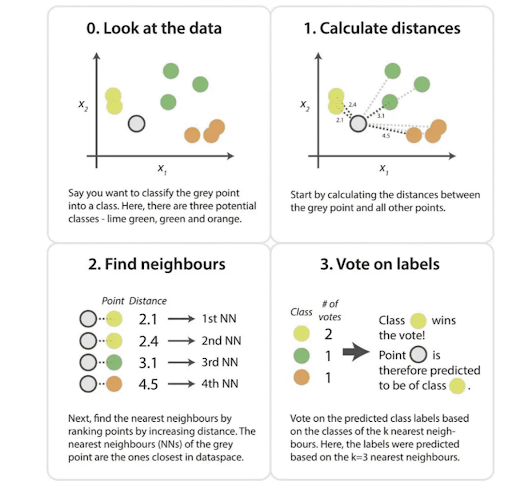
\includegraphics[width=3.125in,height=3.125in]{images/knnimage1.png}

}

\caption{A simple illustration of kNN}

\end{figure}%

Because kNN does not assume any particular distribution of the data, it
is considered non‑parametric. This flexibility makes it easy to apply,
but it also introduces challenges in high‑dimensional spaces where
distances lose contrast, a phenomenon known as the curse of
dimensionality (\citet{kramer2013}, pg 19). (Still don't fully
understand the phenomenon. will return to explain when I do)

\subsection{\texorpdfstring{\textbf{How kNN Works in Recommender
Systems}}{How kNN Works in Recommender Systems}}\label{sec-rec}

In recommendation settings, the task is to predict missing entries in a
sparse user--item matrix of size (number of users) × (number of items).
Each row represents a user, each column an item, and most cells are
empty because users interact with only a small fraction of available
items. Below is an example of such matrix:

\begin{longtable}[]{@{}lllll@{}}
\toprule\noalign{}
User / Item & A & B & C & D \\
\midrule\noalign{}
\endhead
\bottomrule\noalign{}
\endlastfoot
U1 & 4 & 4 & ? & 3 \\
U2 & 4 & 5 & 2 & ? \\
U3 & ? & 4 & 4 & 3 \\
U4 & 2 & ? & 5 & ? \\
\end{longtable}

Since most cells are empty, kNN adapts by computing similarities only on
overlapping ratings. This reliance on shared ratings is both a strength
because it uses actual behavioral similarity and a weakness because
sparsity may cause the similarities to be unreliable
(\citet{kramer2013}). Two main variants are used:

\begin{itemize}
\tightlist
\item
  \textbf{User‑based kNN:} The system identifies the \emph{k} users most
  similar to the target user and infers preferences from their ratings.
  For example, if User 1 and User 2 have rated many of the same items
  similarly, then User 2's rating of a new item can help predict User
  1's interest.
\item
  \textbf{Item‑based kNN:} Instead of comparing users, the system finds
  items that consistently receive similar ratings across users. If Item
  A and Item B are rated alike by many users, then a user who liked Item
  A is predicted to enjoy Item B as well. Item‑based kNN is often more
  stable because item relationships remain consistent even as new users
  enter or leave the system. For this reason, modern commercial
  recommenders tend to use item-based kNN over user-based
  (\citet{ricci2022}).
\end{itemize}

Similarity metrics are central to these computations. \textbf{Cosine
similarity} measures the angle between rating vectors, which makes it
resistant to differences in rating scales. \textbf{Pearson correlation}
adjusts for user biases by centering ratings around individual means.
\textbf{Adjusted cosine similarity} , which is commonly used in
item‑based kNN, subtracts user averages before computing similarity to
reduce the effect of rating habits (\citet{aggarwal2016}). (Should I
include the formulas for computing the 3 similarity metrics?)

Once similarities are computed, predictions are made using weighted
averages. For user‑based kNN, Aggarwal (\citet{aggarwal2016}) defines
one formula for the predicted rating of user (u) for item (i) as:

\[
\hat{r}_{u,i} = \mu_u + \frac{\sum_{v \in P_k(u)} \text{sim}(u,v) \cdot (r_{v,i} - \mu_v)}{\sum_{v \in P_k(u)} |\text{sim}(u,v)|}
\]

Where; (need to explain what each variable in the formula means)

This version adjusts for differences in rating scale by centering
ratings around each user's mean. For item‑based kNN, the formula is
analogous (\citet{aggarwal2016}):

\[
\hat{r}_{u,i} = \frac{\sum_{j \in N_k(i)} \text{sim}(i,j) \cdot r_{u,j}}{\sum_{j \in N_k(i)} |\text{sim}(i,j)|}
\]

Where; (Also need to explain what each variable in the formula means)

Here, the prediction is a weighted average of the user's ratings on
similar items.

These formulas emphasize closer neighbors more heavily thus ensuring
that predictions reflect the most relevant similarities.

\subsubsection{\texorpdfstring{\textbf{Toy
Example}}{Toy Example}}\label{toy-example}

We finish with a toy example adapted from Aggawral's book to emphasize
idea. Consider a simple dataset of three users and three movies:

\begin{longtable}[]{@{}llll@{}}
\toprule\noalign{}
User & A & B & C \\
\midrule\noalign{}
\endhead
\bottomrule\noalign{}
\endlastfoot
U1 & 5 & 4 & ? \\
U2 & 4 & 4 & 2 \\
U3 & 1 & 1 & 1 \\
\end{longtable}

Suppose we want to predict U1's rating for Movie C. First, we compute
the similarity between Movie A and Movie C using cosine similarity:

\[
\text{sim}(A,C) = \frac{(4 \cdot 2) + (1 \cdot 1)}{\sqrt{4^2+1^2} \cdot \sqrt{2^2+1^2}} \approx 0.98
\]

Since U1 rated Movie A highly (5), and Movie A is very similar to Movie
C, the predicted rating for U1 on Movie C is close to 5. This simple
calculation illustrates how kNN leverages neighborhood information to
fill in missing ratings.

\subsection{\texorpdfstring{\textbf{Strengths and Weaknesses of kNN in
Recommendation
Systems}}{Strengths and Weaknesses of kNN in Recommendation Systems}}\label{strengths-and-weaknesses-of-knn-in-recommendation-systems}

As we established in the sections above, kNN requires no training phase,
is easy to explain, and works well for small or dense datasets where
overlaps are plentiful. Its neighbor‑driven reasoning makes it
particularly suitable for educational settings and for systems where
interpretability is valued.

However, kNN also has notable weaknesses. Its reliance on overlapping
ratings makes it vulnerable to sparsity, and its computational cost
grows quickly with dataset size. In high‑dimensional rating matrices,
distance metrics can become unreliable therefore reducing accuracy.
These limitations explain why kNN is often used as a baseline method,
while large‑scale commercial systems rely on more advanced model‑based
approaches such as matrix factorization or deep learning
(\citet{hssina2021}).

\section{\texorpdfstring{\textbf{Comparison to a Model-Based Method
(SVD)}}{Comparison to a Model-Based Method (SVD)}}\label{comparison-to-a-model-based-method-svd}

\begin{itemize}
\tightlist
\item
  What SVD does (very high level) - Use Hssina's article for this
\item
  How it differs from kNN
\item
  Strengths and weaknesses of both
\item
  Maybe Table comparison ?
\item
  When to choose kNN vs SVD
\item
  Why SVD is dominant in large-scale systems
\end{itemize}

\section{\texorpdfstring{\textbf{Application: Building a Simple
Recommendation Engine with
kNN}}{Application: Building a Simple Recommendation Engine with kNN}}\label{application-building-a-simple-recommendation-engine-with-knn}

\subsection{\texorpdfstring{\textbf{Dataset Description + Data
Wrangling}}{Dataset Description + Data Wrangling}}\label{dataset-description-data-wrangling}

\subsection{\texorpdfstring{\textbf{Implementing kNN + Model
Evaluation}}{Implementing kNN + Model Evaluation}}\label{implementing-knn-model-evaluation}

\subsection{\texorpdfstring{\textbf{Results +
Interpretation}}{Results + Interpretation}}\label{results-interpretation}

\section{\texorpdfstring{\textbf{Reflection
(?)}}{Reflection (?)}}\label{reflection}

\section{\texorpdfstring{\textbf{Conclusion}}{Conclusion}}\label{conclusion}

\section{\texorpdfstring{\textbf{Appendix}}{Appendix}}\label{appendix}


\renewcommand\refname{\textbf{References}}
  \bibliography{bibliography.bib}



\end{document}
